\documentclass[twoside]{article}

\usepackage[sc]{mathpazo} 
\usepackage[spanish, es-tabla]{babel}
\usepackage[utf8]{inputenc}

\usepackage[hmarginratio=1:1,top=32mm,columnsep=20pt]{geometry} % Document margins
\usepackage{multicol} % Used for the two-column layout of the document
\usepackage[hang, small,labelfont=bf,up,textfont=it,up]{caption} % Custom captions under/above floats in tables or figures
\usepackage{mathtools}
\usepackage{float} % Required for tables and figures in the multi-column environment - [H] needed
\usepackage{hyperref} % For hyperlinks in the PDF with labels

\usepackage{abstract} % Allows abstract customization
\renewcommand{\abstractnamefont}{\normalfont\bfseries} % Set the "Abstract" text to bold
\renewcommand{\abstracttextfont}{\normalfont\small\itshape} % Set the abstract itself to small italic text

\usepackage{titlesec} % Allows customization of titles

\titleformat{\section}[block]{\large\scshape\centering}{\thesection.}{1em}{} % Change the look of the section titles
\titleformat{\subsection}[block]{\large}{\thesubsection.}{1em}{} % Change the look of the section titles

\usepackage{fancyhdr} % Headers and footers
\pagestyle{fancy} % All pages have headers and footers
\fancyhead{} % Blank out the default header
\fancyfoot{} % Blank out the default footer
\fancyhead[C]{Caracterización de un diodo PIN% based on TRACS 
\hspace{4pt} $\bullet$ \hspace{4pt} Enero 2019 } % Custom header text
\fancyfoot[RO,LE]{\thepage} % Custom footer text

%----------------------------------------------------------------------------
%	   TITLE SECTION
%----------------------------------------------------------------------------

\title{
	\vspace{-15mm}
	\fontsize{18pt}{10pt}
	\selectfont\textbf{Técnica de corriente transitoria (TCT) para la caracterización de un diodo PIN semiconductor usando un láser de 670 nm}% Article title
}

\author{
	\large
	\textsc{Jaime D\'iez Gonz\'alez-Pardo}\\[4mm]
	\fontsize{28pt}{10pt} Universidad de Cantabria \\ % Your institution
	%\thanks{A thank you or further information}\\[2mm] % Your name
	\normalsize Física de Partículas \\ 
	%\normalsize{Compañeros:} \textsc{NOMBRE COMPANEROS }\\%\normalsize \href{mailto:john@smith.com}{john@smith.com} % Your email address
	%\vspace{5mm}
}

\date{ \today }


%----------------------------------------------------------------------------
%      · DOCUMENT
%----------------------------------------------------------------------------

\begin{document}


	\maketitle % Insert title


	\thispagestyle{fancy} % All pages have headers and footers

%----------------------------------------------------------------------------
%	  ARTICLE CONTENTS
%----------------------------------------------------------------------------


	\section{Ejercicio 1}
		\label{sec:ej1}
						 
		Cuando se ilumina la superficie de un semiconductor con un láser se libera energía al material, produciendo la creación de pares electrón-hueco a medida que el láser penetra en él. Para los láseres rojos, se tiene que la  capacidad de penetración es baja, por lo que no llegará a penetrar mucha profundidad en el material, creando los pares electrón-hueco solo en las zonas cercanas a la superficie iluminada, siendo la zona afectada de unos pocos micrómetros para el caso del silicio. 

		En el caso del ejercicio se trata de un láser rojo que ilumina un diodo PIN con una parte dopada $n$, exceso de electrones, y una parte dopada $p$, exceso de huecos. Como se ha dicho, el láser rojo solo penetrará unos pocos micrómetros en el diodo, produciendose la creación de pares electrón-hueco solo en la zona dopada $n$ o en la zona dopada $p$, dependiendo que superficie sea iluminada.

		Hay que tener en cuenta, que en el caso del diodo PIN, la zona del dopaje $n$ está conectada al electrodo negativo, y la zona del dopaje $p$ al electrodo positivo. Debido a esto, si la parte iluminada es la zona con dopaje $n$, los electrones producidos en la creación de pares electrón-hueco, serán absorvidos por el electrodo negativo, quedando solo libres los huecos. Esto es equivalente a decir que se inyectan huecos en el diodo. Si por el contrario la superficie iluminada es la dopada $p$, serán los hucos de los pares electrón-hueco los que sean absorvidos por el electrodo positivo, siendo equivalente a inyectar electrones en el diodo.

	\section{Ejercicio 2}

		\subsection{Ejercicio 2.a)}
			\label{sec:2a}

			En el ejercicio se dice que se  tiene una unión p-n con la región $n^+$ mucho más dopada con impurezas, siendo $N_{donadores} >> N_{aceptadores}$. De esta forma se sabe que la densidad de carga ha de ser igual a $\rho = e(N_{donadores} - N_{aceptadores})$, siendo $e$ la carga del electrón. De las ecuaciones de Maxwell se puede obtener, a partir de la forma diferencial de la ley de Gauss, la siguiente ecuación de Poisson:

				\begin{equation}
					\nabla E = \frac{\rho}{\epsilon}
					\label{eq:piosson}
				\end{equation}

			Resolviendo dicha ecuación para un sistema unidimensional se puede obtener la siguiente ecuación:

				\begin{equation}
				\begin{matrix}
					\nabla E = \frac{\rho}{\epsilon} \equiv \frac{\mathrm{d} E}{\mathrm{d} x} = \frac{\rho} {\epsilon}\Rightarrow\mathrm{d} E = \frac{\rho} {\epsilon} \mathrm{d} x
					\\
					\\
					\int \mathrm{d}E = \frac{\rho}{\epsilon}\int \mathrm{d}x \Rightarrow E = \frac{\rho} {\epsilon} x = \frac{xe(N_{donadores} - N_{aceptadores})}{\epsilon}
					\end{matrix}
				\end{equation}

		\subsection{Ejercicio 2.b)}
			\label{sec:2b}

			Otra forma de obtener el campo eléctrico es a partir del potencial eléctrico, ya que se sabe que el campo es igual a menos el gradiente del potencial eléctrico ($E = -\nabla \phi$). Teniendo en cuenta las consideraciones del apartado \ref{sec:2a} y la ecuación \ref{eq:piosson}, se puede obtener que:

				\begin{equation}
					\frac{\mathrm{d}V} {\mathrm{d}x} = E = \frac{e N} {\epsilon} x
					\label{eq:poisson2}
				\end{equation}

			No obstante debemos tener en cuenta que la ecuación \ref{eq:poisson2} ha de cumplirse para las dos regiones que se tienen, tanto la de donadores como la de aceptadores, sustituyendo la $N$ por la concentración de cada uno. Además, hay que tener en cuenta que el campo ha de anularse en la zona de agotamiento, siendo $x \rightarrow (x \pm x_i) \textrm{ con } i = n, p$.

				\begin{equation}
					\begin{matrix}
						\frac{\mathrm{d}V} {\mathrm{d}x} = E = \frac{e \cdot  
						\begin{Bmatrix}
							N_{aceptadores} \\ N_{donadores}
						\end{Bmatrix}} {\epsilon}\left(x +  
						\begin{Bmatrix}
							x_p \\ -x_n
						\end{Bmatrix}\right)

						\\
						\\

						V  = \int E \mathrm{d}x = \int \frac{e \cdot  
						\begin{Bmatrix}
							N_{aceptadores} \\ N_{donadores}
						\end{Bmatrix}} {\epsilon}\left(x +  
						\begin{Bmatrix}
							x_p \\ -x_n
						\end{Bmatrix}\right)\mathrm{d}x

						\\
						\\

						V_{bias} = \frac{e \cdot  } {2\epsilon}
						\begin{Bmatrix}
							N_{aceptadores} \\ N_{donadores}
						\end{Bmatrix} \left(x +  
						\begin{Bmatrix}
							x_p \\ -x_n
						\end{Bmatrix}\right)^2
					\end{matrix}
					\label{eq:desarrollo}
				\end{equation}

			Despejando la componente de las $x$ del desarrollo \ref{eq:desarrollo} se pueden obtener las profundidades de agotamiento tanto para el dopaje $n$ como para el $p$.

				\begin{equation}
					\begin{matrix}
						(x + x_p) = \sqrt{\frac{V_{bias}2\epsilon}{eN_{aceptadores}}}

						\\
						\\

						(x - x_n) = \sqrt{\frac{V_{bias}2\epsilon}{eN_{donadores}}}
						
					\end{matrix}
				\end{equation}

		\subsection{Ejercicio 2.c)}
			\label{sec:2c}

			A partir del desarrollo realizado en el apartado anterior \ref{sec:2b} y tomando los datos que facilitados por el ejercicio se puede obtener el $V_{bias}$. Para realizar el calculo correcto se ha de tener en cuenta que se trata de un dopado $p$, por lo que $\rho = 1/ e N \mu_H$, siendo $\mu_H$ la movilidad de los huecos.  

				\begin{equation}
					\begin{matrix}
						\begin{matrix}
							\left.\begin{matrix}
								(x+x_p) = 300 \mu m = 3 \cdot 10^{-4} m
								\\
								\mu_H = 450 cm^2 /(Vs) = 0.045 m^2 /(Vs)
								\\
								\rho = 30 k\Omega cm = 300 \Omega m
							\end{matrix}\right\}
							&
							V_{bias} = \frac{eN_{aceptadores}}{2\epsilon} (x+x_p)^2 = \frac{1}{2\epsilon\rho\mu_H} (x+x_p)^2
						\end{matrix}
						\\ \\
						V_{bias} = \frac{1}{2\epsilon \cdot 300 \cdot 0.045} (3 \cdot 10^{-4})^2 = 376.47 V
					\end{matrix}
				\end{equation}

	\section{Ejercicio 3}

		\begin{figure}[H]
			\centering
			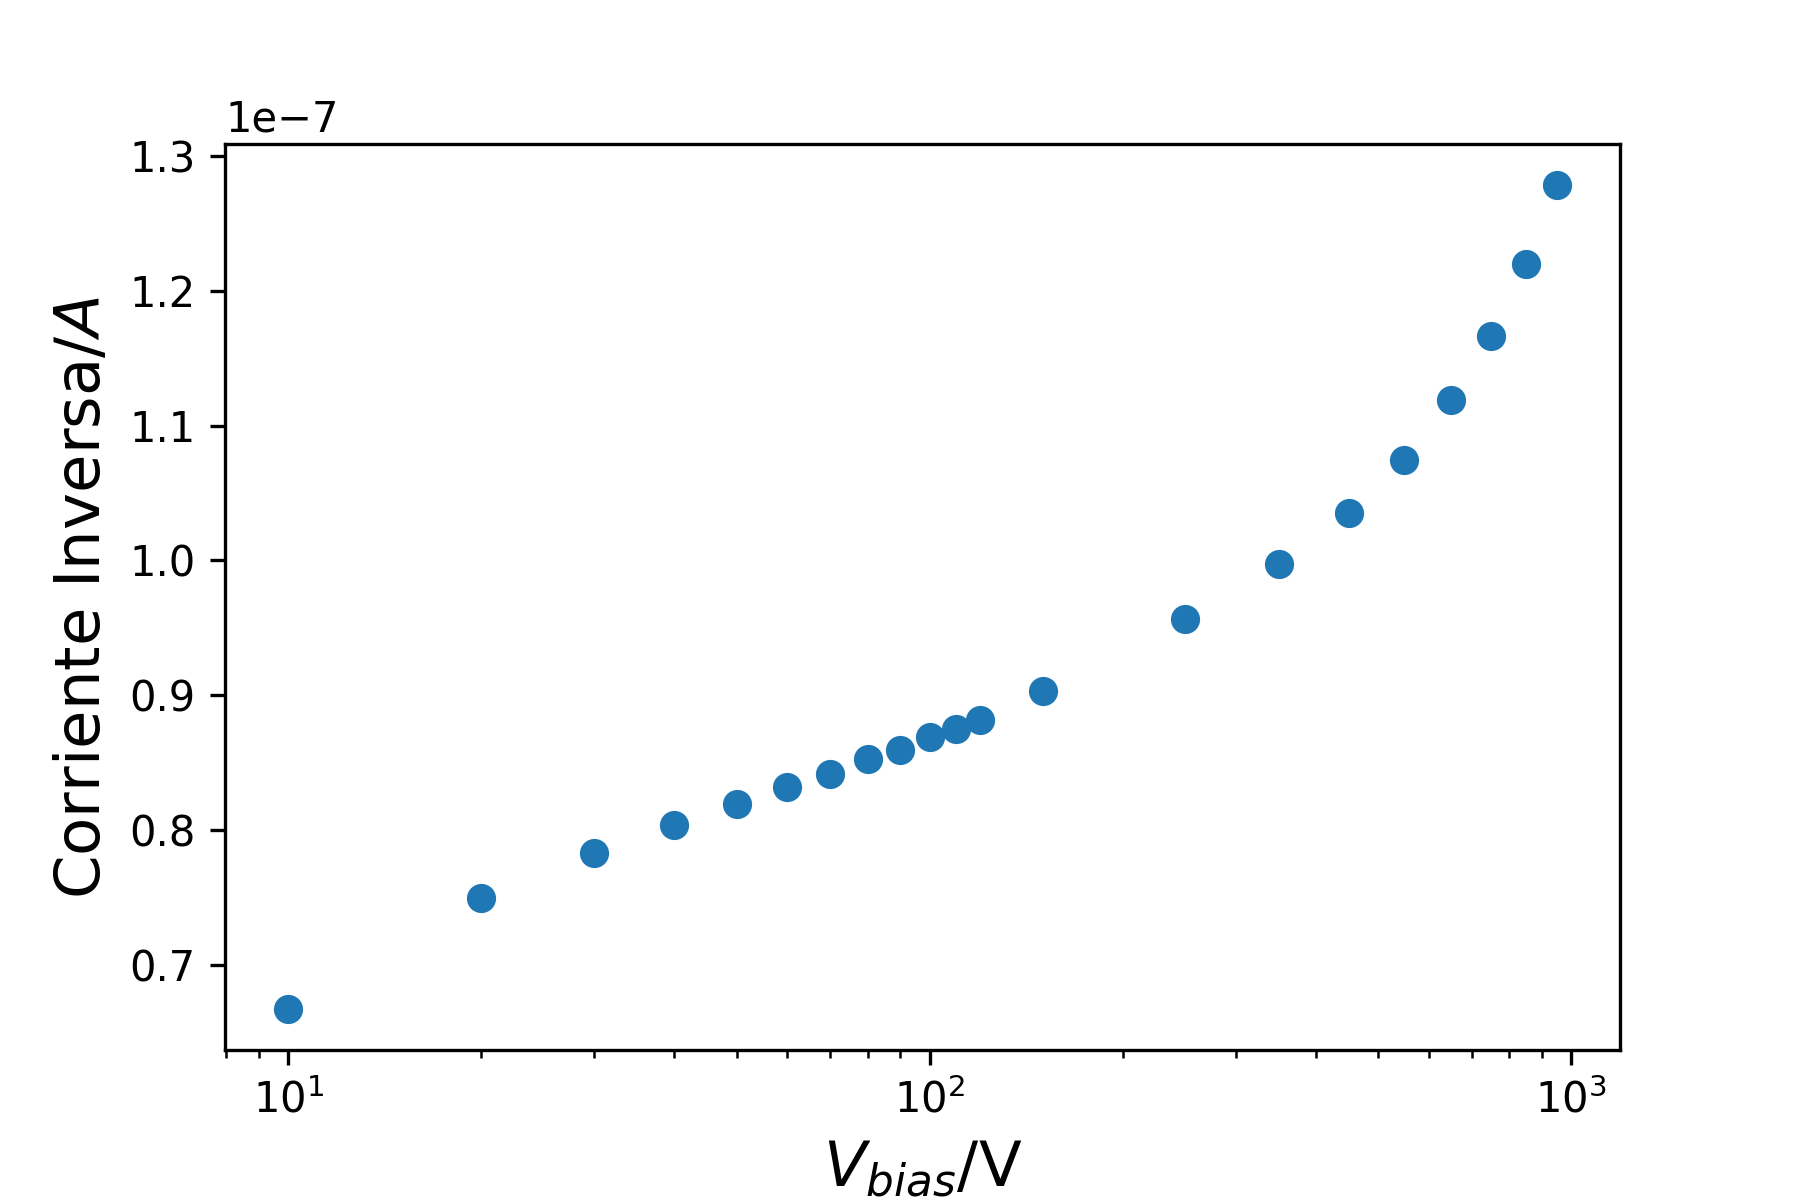
\includegraphics[scale=0.8]{todos.png}
			\caption{\label{Img:I-V}Corriente inversa frente al voltaje $V_{bias}$. Los voltajes se representan en escala logaritmica.}
		\end{figure}

		En la Figura \ref{Img:I-V} se representan la corriente inversa frente al voltaje, representando estos últimos en escala logaritmica. Al tratarse de corriente inversa, estamos en polarización inversa y los pares electrón-hueco son generados por energía térmica. Cuando estos electrones y huecos generados pierden dicha energía térmica se produce una corriente inversa de saturación. Este fenómeno corresponde a los con voltaje $V_{bias}$ de entre 10-100 V  de la Figura \ref{Img:I-V}, donde se encuentra una mayor concentración de puntos. Es precisamente en esta zona en la que se realiza un promedio del valor de la intensidad, obteniendo un valor de $\bar{I} = (8.0 \pm 0.6) \cdot 10^{-8} A$. Con este valor y conociendo las dimensiones de diodo dadas en la guía de la práctica \cite{guia} se puede obtener la corriente inversa por unidad de volumen.

			\begin{equation}
				I/V{olumen} = \frac{(8.0 \pm 0.6) \cdot 10^{-8}}{(5\cdot 10^{-3})^2\cdot (300 \cdot 10^{-6})} = (10.7 \pm 0.8) A/m^3
			\end{equation}
	
	\section{Ejercicio 4}

		\subsection{Inyección de Electrones}

			Tal y como se ha visto en el Ejecicio 1 \ref{sec:ej1}, la inyección de electrones es debido a que el láser rojo ilumina la superficie dopada $p$ situada en el electrodo positivo. Puesto que esto equivale a la aparición de electrones espontaneamente en el diodo, se producirá un aumento de la corriente que podrá ser detectada (negativa debido al criterio utilizado). Esto se verá reflejado en la gráfica como una caida rápida de la corriente. Tras esto, el electrón tratará de moverse al otro electrodo. Al producirse dicho electrón en una zona con bajo campo eléctrico y moverse hacia zonas con mayor campo eléctrico, su velocidad de arrastre aumentará, por lo que la corriente también lo hará. En la gráfica se obserevará una zona de pendiente constante, que según nuestro criterio de signos tendrá pendiente negativa. Por último, el elctrón será absorvido por el electrodo negativo y el diodo volverá a su estado inicial.

			En la Figura \ref{Img:ejemploE} se muestra una gráfica del voltaje detectado al inyectar electrones en el diodo. En dicha gráfica se observan claramente las 3 zonas mencionadas.

				\begin{figure}[H]
					\centering
					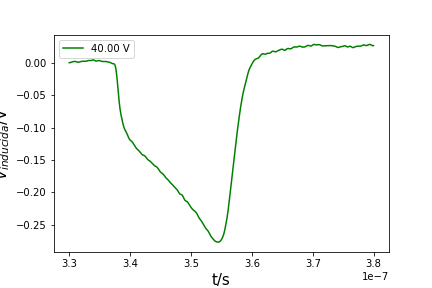
\includegraphics[scale=0.8]{Ejemplo.png}
					\caption{\label{Img:ejemploE}Voltaje detectado al inyectar electrones en el diodo en función del tiempo.}
				\end{figure}

		\subsection{Inyección de Huecos}

			En este caso, según el Ejercicio 1 \ref{sec:ej1}, el láser ilumina la parte del dopado $n$, creando huecos en la parte del electrodo negativo. De igual manera que en la inyección de electrones, se deberá observar un aumento repentino de la corriente, que corresponderá con una caida del voltaje en la gráfica. Sin embargo, en este caso los huecos, con una velocidad de arrastre mucho menor que los electrones, son creados en la zona en la que el campo eléctrico es máximo, trantando de moverse hacia el electrodo positivo con un campo menor. Esto producirá una disminución en la corriente. En la gráfica lo que se observará será una pendiente similar a la de la inyección de huecos, pero con pendiente contraria ya que su velocidad disminuirá.

	\section{Ejercicio 5}

		\begin{equation}
			\begin{matrix}

				\textrm{Impedancia} \rightarrow Z = 50 \Omega & & & &  \textrm{Ganancia} \rightarrow 60 dB
			\end{matrix}
		\end{equation}

		\subsection{Ejercicio 5.a)}

			En el fichero de Datos facilitado para el escaner fino se encuentran los voltajes inducidos en el diodo en función de tiempo para diferentes voltajes de agotamiento. En la Figura \ref{Img:fina} se muestran dichos datos con lo perfiles del voltaje. A partir de dicha gráfica se observa que el voltaje $V_{bias}$ ha de ser de $30 V$.

				\begin{figure}[H]
					\centering
					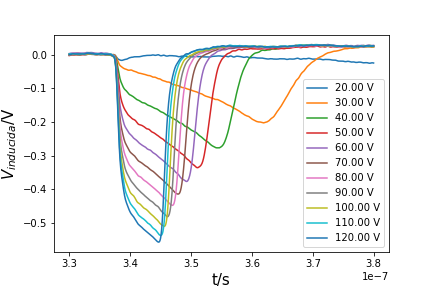
\includegraphics[scale=0.8]{fina.png}
					\caption{\label{Img:fina}Voltajes inducidos en el diodo en función de tiempo para diferentes voltajes de agotamiento}
				\end{figure}

			Se sabe que el voltaje está relacionado con la intensidad de corriente a través de la impedancia de la forma $I = V/Z$, por lo que dichos perfiles son proporcionales a la intensidad. Sabiendo además que la carga se define como $\mathrm{d}Q = I \mathrm{d}t$, se puede sacar ésta como la integral de $I$ a lo largo de $t$, o lo que es lo mismo, el área que encierra dicho perfil.

			En la figura \ref{Img:Q} se muestran los valores de la carga obtenidos a partir de la integral de $I$, para cada uno de los voltajes de agotamiento.

				\begin{figure}[H]
					\centering
					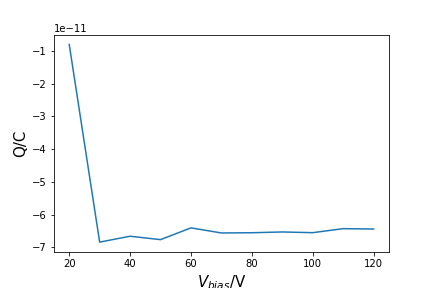
\includegraphics[scale=0.8]{Q.png}
					\caption{\label{Img:Q}Valores de la carga obtenidos a partir de la integral de $I$, para cada uno de los voltajes de agotamiento.}
				\end{figure}

		\subsection{Ejercicio 5.b)}

			De la Figura \ref{Img:fina} del apartado anterior se obtiene que el voltaje de agotamiento ha de ser $V_{bias} = 30 V$. Si tomamos el desarrollo realizado en los apartados \ref{sec:2b} y \ref{sec:2c} y  tomando el dato $(x - x_n) = (x + x_p) = 300 \mu m$ se puede obtener un valor para la concentración de impurezas en el diodo. Puesto que hemos supuesto $(x - x_n) = (x + x_p)$, este resultado será valido tanto para las impurezas de tipo $n$ como  para las $p$.

				\begin{equation}
					N = \frac{2\epsilon_0 V_{bias}}{e(x - x_n)^2} = \frac{2\epsilon_0 30}{e(3 \cdot 10^{-4})^2} = 3.68 \cdot 10^{16} \textrm{impurezas} / m^3
				\end{equation}

		\subsection{Ejercicio 5.c)}

			Se sabe que se tiene un láser rojo cuya longitud de onda es $\lambda = 670 nm$, por lo que la energía del haz ha de ser:

				\begin{equation}
					E = \frac{hc}{\lambda} = 1.85 eV
				\end{equation}

			Por otro lado, a partir de los valores de la carga de la Figura \ref{Img:Q}, y teniendo en cuenta el factor de amplificación de $1000$, se puede obtener el valor medio de la carga, siendo de $\bar{Q} = 6.05 \cdot 10^{-14} C = 377749 e$. Esto quiere decir que la carga inducida en el diodo equivale a la carga de $377749$ electrones, aunque en este caso se ha de considerar que dicha carga proviene no solo de los electrones si no, de igual manera, de los huecos, considerando que no se producen recombinaciones. De esta forma, el número de pares electrón-hueco sería:

				\begin{equation}
					n_{e-h} = 377749 / 2 = 188874
				\end{equation}

			Con esto, conocida la energía de los fotones incidentes, y que la energía de creación del par electrón-hueco en el silicio es $E_{e-h} = 3.6 eV \approx 2E $ \cite{nickname}, y conocido el numero de pares electrón-hueco creados, se puede conocer la energía emitida por el láser.

				\begin{equation}
					E_{laser} = n_{e-h} \cdot 2 \frac{hc}{\lambda} = 0.7 MeV
				\end{equation}

%----------------------------------------------------------------------------
%     BIBLIOGRAPHY
%----------------------------------------------------------------------------

	\bibliographystyle{unsrt}
	\bibliography{biblio}

\end{document}

%----------------------------------------------------------------------------
%            TEMPLATES
%----------------------------------------------------------------------------

%----------------------------------------------------------------------------
%            how to insert an image
%----------------------------------------------------------------------------

%	\begin{figure}[H]
%		\centering
%		\includegraphics[scale= ]{nombre de la imagen.jpg}
%		\caption{\label{Img:widgets}el pie de pagina que le quieras 	poner a la imagen}
%	\end{figure}
 
%----------------------------------------------------------------------------
%            how to insert a table
%----------------------------------------------------------------------------

%	\begin{table}[H]
%		\centering
%		\begin{tabular}{|c|c|c|c|}
%			\hline
%			\centering
%				Altura(h) & Distancia (d) & Elaboracion (e) & Longitud (l) \\
%				($\pm0.5$ mm) & ($\pm0.5$ mm) & ($\pm0.5$ mm) & ($\pm0.5$ mm) \\ \hline
%				 &  &  &  \\ \hline
%				 &  &  &  \\ \hline
%				 &  &  &  \\ \hline
%				 &  &  &  \\ \hline
%				 &  &  &  \\ \hline
%		         &  &  &  \\ \hline
%		\end{tabular}
%		\caption{\label{Tab:widgets}pie de pagina que le quieras poner}
%	\end{table}

%----------------------------------------------------------------------------
%             How to remove the label in equactions
%----------------------------------------------------------------------------

%	\begin{equation*}
%		
%	\end{equation*}

%----------------------------------------------------------------------------
%              How to set bibliography
%----------------------------------------------------------------------------

%\bibliographystyle{unsrt}
%\bibliography{biblio}
%
%Then you have to set a .bib document such as the next template
%
%	@book{nickname,
%	author = {},
%	title = {},
%	edition = {},
%	year = {},
%	volume = {},
%	ISBN = {}
%	}
%
%	@ARTICLE{nickname,
%	author = {},
%	title = {},
%	year = {},
%	volume = {},
%	}


%----------------------------------------------------------------------------
%              END
%----------------------------------------------------------------------------
